\chapter{Моделирование TGE и TGF
}\label{ch:thunderstorm}

\section{Обзор экспериментальных результатов
}\label{sec:thunderstorm/review-exp}


% Статья Chubenko2000.pdf - наблюдение рентгеновского излучения на Тяньшане
% Статья Chubenko2003.pdf - рост числа электронов в спокойной фазе без вспелесков гамма-квантов на Тяньшане
% Статья Chubenko2009.pdf - измерение спектра TGF на Земле
% Статья Antonova2007.pdf - появление радиосигналов при прохождении ШАЛ через грозу, в отсутвии ШАЛ радиосигнала нет.
% Статья Antonova2009.pdf - появление радиосигналов и гамма эмиссии скорелированной с прохождением ШАЛ через грозу и разрядами, в отсутвии ШАЛ радиосигнала нет.
% Gurevich2000.pdf --- даны оценки числа рожденных электрон-позитронных пар
% Gurevich_etal2013.pdf - Приведены результаты одновременных измерений радио и гамма-излучения во время гроз. Гамма-детектор, расположенный на высоте 3840 м, и два радиодетектора Тянь-Шаньской горной научной станции (высота 3340 м) регистрировали интенсивные гамма-вспышки и радиоимпульсы в момент возникновения молнии. В начальный момент времени (несколько сотен микросекунд) радиогамма-корреляция резко нарастает, а коэффициент корреляции достигает 0,9–0,95. Спектр гамма-энергии, измеренный при возникновении молнии, близок к характерному спектру пробоя на убегающих электронах. Наблюдаемые при этом радиоимпульсы имеют наибольшую амплитуду. Совместное наблюдение гамма-излучения и радиоизлучения подтверждает концепцию возникновения молнии из-за множественных одновременных электрических разрядов на гидрометеорах, стимулированных и синхронизированных низкоэнергетическими электронами, генерируемыми в процессе разгона. 
% Gurevich2001.pdf -- рсчеты гуревича для неоднороного поля, добавить в раздел про реактор
% Gurevich2002.pdf ---расчеты Гуревича для радиоимпульса от ШАЛ в грозе
% Gurevich2003.pdf --- наблюдение радиосигнала соотвевующего расчетам из Gurevich2002.pdf 
% Gurevich2011_background.pdf --- наблюдения TGF на Тянь-Шане.

\section{Обзор существующих моделей}\label{sec:thunderstorm/review-mod}

\subsection{Пробой на убегающих электронах}\label{sec:thunderstorm/gurevich}
%
Пробой на убегающих электронах (ПУЭ) --- модель развития лавины релятивистских (с энергией 0.1 --- 10 МэВ) электронов в постоянном электрическом поле предложенная А.~В.~Гуревичем~\cite{gurevich1992runaway,Gurevich2001ufn}. Качественно идея модели проста: пусть электрон ускоряется за счет электрического поля и тормозится за счет взаимодействия со средой, если он получает от поля больше энергии чем теряет, то у него появляется избыток энергии, который может быть потрачен на рождение нового электрона. Такие электроны будем называть убегающими. Если пренебречь всеми процессами кроме ионизационных потерь и радиационных потерь, то график ~\ref{fig:storm:gurevich}а показывает условия генерации лавины убегающих электронов в однородном поле. Энергию при которой электрон в среднем на единице длинны приобретает энергии больше чем теряет мы будем называть критической (зависимость её от высоты\footnote{Если не указано иное, Для установления значения плотности воздуха на разных высотах в моделировании используется международная стандартная модель атмосферы (ISA)} приведена на рис. ~\ref{fig:storm:gurevich}б).

\begin{figure}[t]
    \begin{center}
        \begin{minipage}[h]{0.49\linewidth}
            \center{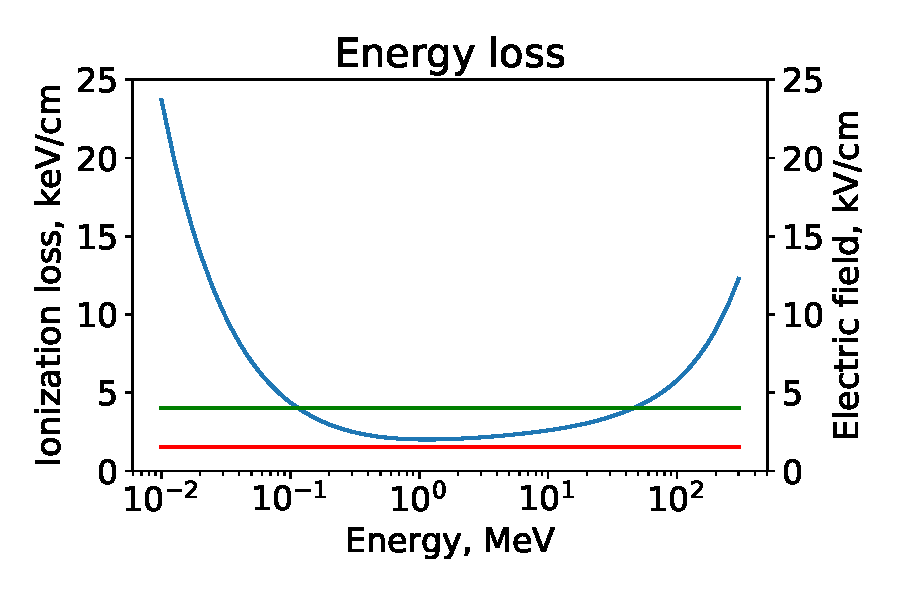
\includegraphics[width=\linewidth]{thunderstorm/01_Gurevich.pdf} \\ а)}
        \end{minipage}
        \hfill
        \begin{minipage}[h]{0.49\linewidth}
            \center{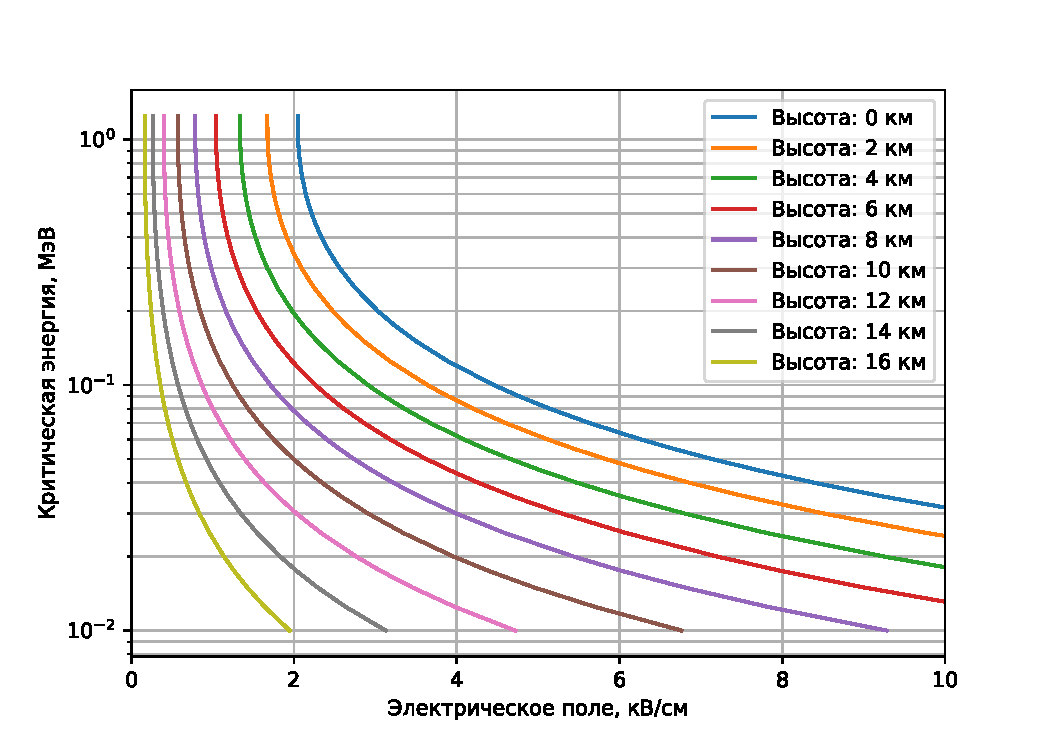
\includegraphics[width=\linewidth]{thunderstorm/02_CriticalEnergy.pdf}   \\ б)}
        \end{minipage}
        \caption{а) Ионизационные потери электронов в воздухе при нормальных условиях. б) Зависимость критической энергии от поля для различных высот.}
    \end{center}
    \label{fig:storm:gurevich}
\end{figure}

\section{Расчет числа убегающих электронов}\label{sec:thunderstorm/rrea}

Простая аналитическая оценка числа убегающих электронов может быть получена из элементарной теории ПУЭ~\cite{Gurevich2001ufn}. Давайте рассмотрим развитие электронной лавины в однородном электрическом поле. Согласно~\cite{Gurevich2001ufn} число убегающих электронов в RREA возрастает экспоненциально вдоль оси z:

\begin{equation}
\label{storm:exp}
N(z) = N_0 \cdot e^{\frac{z}{l_a}},
\end{equation}

где $l_a$ --- характерная длина нарастания электронной лавины, которая может быть оценена по следующей формуле:

\begin{equation}
l_a = a\frac{2 m c^{2}}{e} \frac{1}{E},
\end{equation}

где $m$ --- масса электрона, $c$ --- скорость света, константа $a \approx 11$, $E$ --- электрическое поле (для электронов с энергиями выше 80 МэВ, начинают доминировать радиационные потери, но тем не менее эта формула может дать оценку сверху). В качестве альтернативы мы можем использовать эмпирическую формулу полученную в стимуляциях Дваера~\cite{Dwyer2007}:

\begin{equation}
\label{storm:dwyer}
l_a = \frac{7300 kV}{E - 276 \frac{kV}{m} \cdot \frac{n}{n_0}},
\end{equation}

где $E$ --- электрическое поле, $n$ - концентрация воздуха, $n_0$ --- концентрация воздуха при н. у. Используя эти формулы, можно рассчитать число релятивистских электронов в зависимости от размера области с поле и величины поля. Результаты расчетов для высоты 10~км представлены на графике ~\ref{storm:number_runway}а, из него видно для максимально возможных условий на данной высоте (регион с полем не превышает 1200~метров, а электрическое поле~200 кВ/м) количество электронов не превышает $10^{10}$.

\begin{figure}[t]
    \begin{center}
        \begin{minipage}[h]{0.49\linewidth}
            \center{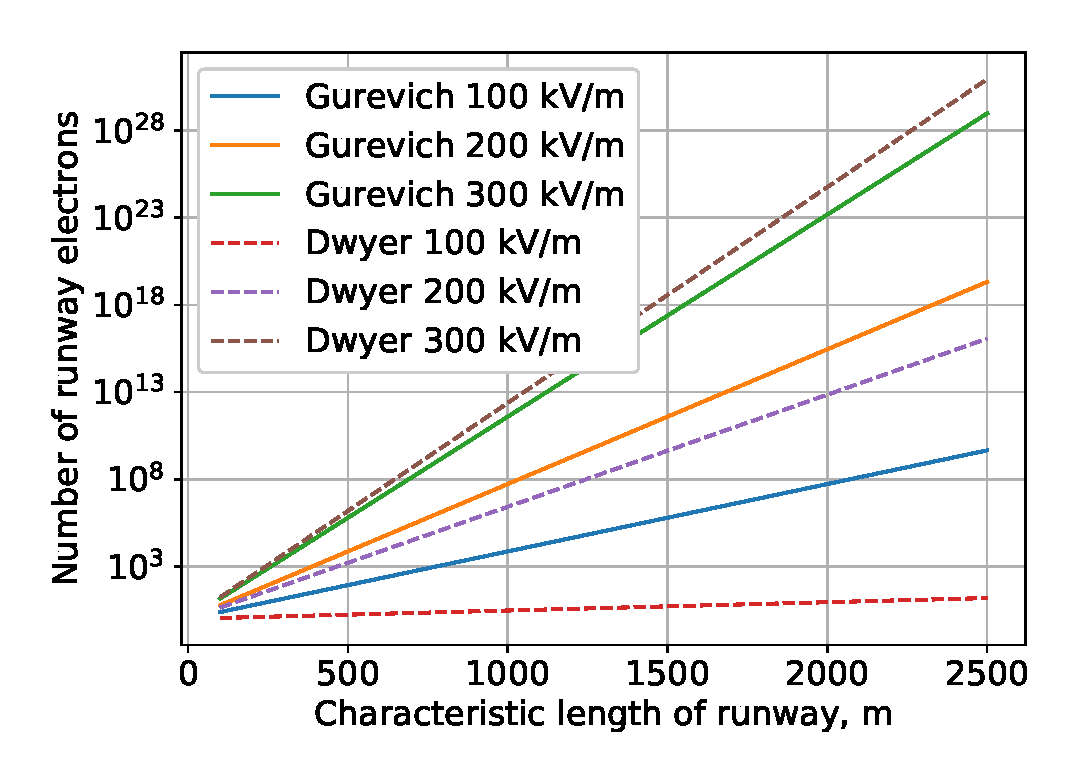
\includegraphics[width=\linewidth]{thunderstorm/epl2020/gurevich.eps} \\ а)}
        \end{minipage}
        \hfill
        \begin{minipage}[h]{0.49\linewidth}
            \center{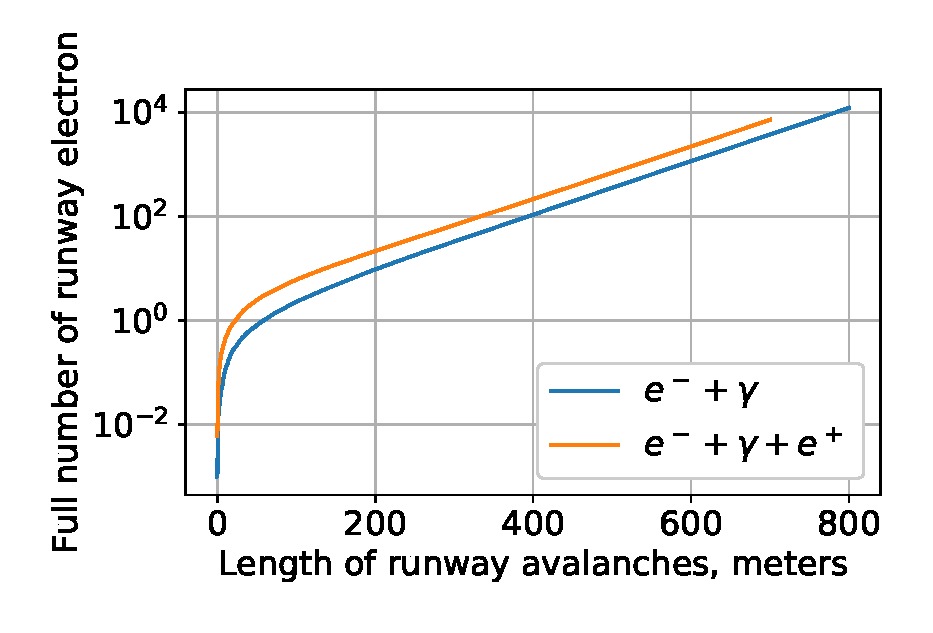
\includegraphics[width=\linewidth]{thunderstorm/epl2020/simulation.eps}   \\ б)}
        \end{minipage}
        \caption{  а) Число убегающих электронов в лавине в зависимости от длинны лавины. б) Число убегающих электронов из GEANT4 симуляции: синяя линия --- симуляция без позитронов, оранжевая --- с позитронами.}
    \end{center}
    \label{storm:number_runway}
\end{figure}
Более точные значения можно получить с помощью Монте-Карло моделирования лавины в электрическом поле с помощью GEANT4~\cite{Geant2003,Geant2006, Geant2016} (в данном разделе приведены расчеты с использованием версии 4.10.05).
Моделирование было проведено для следующих параметров: 
\begin{itemize}
    \item Область с полем представляет собой  цилиндр с шириной много большей его толщины, электрическое поле и плотность воздуха однородны;
    \item Плотность воздуха --- 0.4~кг/м~$^3$ (соответствует атмосферному давлению в  $\sim 0.25$~атм или высоте 10~км от уровня моря);
    \item Электрическое поле --- $200$~кВ/м (это максимальное электрическое поле обычно измеряемое в облаках~\cite{rakov_uman});
    \item Размер области с полем --- $800$~м для симуляции без позитронов и $700$~м для симуляции с позитронами (как мы увидим позже эти длины примерно соответствуют 10 характерным длинам нарастания лавины, что позволяет признать эти длины достаточными);
    \item Минимальный порог для рождения частиц --- 0.05 МэВ.
\end{itemize}
В каждой симуляции запускалось 1000 затравочных электронов (конечные результаты приведены на один электрон), результат симуляции приведен на рисунке~\ref{storm:number_runway}б. Результаты были фитированы функцией ~\ref{storm:exp}, в результате чего получены значения  $l_a \approx 85 m$ для симуляции без позитронов и $l_a \approx 78~m$ для симуляции с позитронами (для сравнения ~Eq.~\ref{storm:dwyer}~(формула Дваера) предсказывает $l_a \approx 64~m$). Используя полученную характерную длину можно оценить число убегающих электронов для разных длин, некоторые характерные значения приведены в таблице~\ref{tab:storm:approx}. На интересном нам участке $1200 - 1700$~метров рождает только $10^6-10^8$ убегающих электронов, что гораздо меньше числа $10^{16}$ предсказываемого в работе~\cite{Oreshkin_2018}, и сравнимо с оценками даваемыми другими авторами.
\begin{table}[h]
    \centering
    \begin{tabular}{crrr}
        \hline
        & & \multicolumn{2}{r}{Число убегающих электронов} \\
        &   Длина, м &   без позитронов &  с позитронами \\
        \hline
        \multirow{4}*{\rotatebox[origin=c]{90}{моделирование}} & 300 &  34.3      &  46 \\
        & 500 &  361     &  589 \\
        & 700 &  3802     &  7539 \\
        & 800 &  12350 &  --- \\
        \hline
        \multirow{5}*{\rotatebox[origin=c]{90}{экстраполяция}}& 1200 &  1.4e+06 &  4.3e+06 \\
        & 1700 &  5.0e+08 &  2.5e+09 \\
        & 2000 &  1.7e+10 &  1.2e+11 \\
        & 4000 &  2.9e+20 &  1.3e+22 \\
        & 5000 &  3.7e+25 &  4.5e+27 \\
        \hline
    \end{tabular}
    \caption{Оценка полного числа убегающих электронов основанная на симуляции в области размером 700-800 метров. Первая часть таблицы это взятые из симуляции, вторая часть это экстраполяция результатов моделирования.}
    \label{tab:storm:approx}
\end{table}


\section{Расчет коэффициента обратной связи, сравнение с результатами Дваера}\label{sec:thunderstorm/rdfm}


\section{Анализ структуры грозового облака на основе наблюдения TGE}
В отличии от TGF представляющие собой очень короткие (~10 мкс) вспышки гамма- и рентгеновского излучения из грозового облака, TGE представляет собой длительное повышение гамма-фона. По результатам наблюдений на горе Арагац академиком Чилингаряном была предложено разделить TGE на две условные группы: 
High Energy Particle TGE (HEP TGE) имеющие длительность порядка нескольких минут и значительную высокоэнергичную (энергия гамма-квантов более 3 МэВ) компоненту и Long-Lasting Low Energy TGE (LLLL TGE) имеющие длительность более двух часов и при этом содержащие в основном низкоэнергитичные (менее 3 МэВ) гамма-кванты. При этом можно отметить следующие особенности: 
\begin{itemize}
    \item HEP TGE  возникает при глубоких  провалах  приповерхностного поля, но не каждый провал сопровождается HEP TGE,
    \item Возможно существование LLLE TGE без  HEP TGE,
    \item Возможно cуществование LLLE TGE при полях ниже поля убегания электронов,
    \item HEP TGE может возникать несколько раз: оно может быть разрушено из-за вспышки молнии и потом восстановится.
\end{itemize}
В контексте изучения возникновения молнии HEP TGE и LLLE TGE интересны, так как они могут помочь описать структуру грозового облака.  Так первым представление об грозовом облаке был вертикальный диполь, однако реальная его структура гораздо сложнее, в данной работе мы рассмотрим генерацию TGE c точки зрения трипольной модели(хотя по всей видимости облака могут иметь и большее число слоев). При представлении облака как вертикального триполя считается что в центре облака собирается отрицательный заряд, в верхней части облака и на земле индуцируется положительный заряд, и наконец в нижней части облака формируется небольшая область с положительным зарядом. Тогда можно сформулировать следующие гипотезы:
\begin{itemize}
    \item Затравочными частицами служат электроны от космических лучей;
    \item LLLE TGE -возникает за счет поля между основным отрицательным зарядом и зарядом индуцированным в земле;
    \item По мере развития нижнего положительного заряда (НПЗ)  возрастает поле и поток частиц в LLLE TGE переходит в HEP TGE;
    \item Регистрация HEP TGE происходит при прохождении НПЗ над детектором
\end{itemize}
Для проверки этих гипотез в работе были проанализированны экспериментальные наблюдения которые сравнивались с моделированием с помошью CORSIKA и GEANT4. Далее приводятся результаты проведенного для этой работы  автором диссертации GEANT4 моделирования. В частности автором были проведенным моделирования превышения гамма-квантов в зависимости от электрического поля, а также получены их угловые и радиальные распределения. Симуляция проводилась при следующих параметрах: первичными частиц являются гамма-кванты в диапазоне энергий от 1 до 100 МэВ, имеющие степенной спектр вида $E^{-1.42}$, начальная точка расположена в тысяче метрах над станцией(которая находится на высоте 3200 метров над уровнем моря), моделирование проводилось в подкритических полях (значение критического поля для данных высот порядка 1.7-1.8 кВ/см
), также моделирование проводилось с использование двух физических листов G4EmPhysStandard и G4EmPhysStandar\_opt4 (использовался GEANT4 версии 4.10.4). График демонстрирует рост потока гамму, даже в подкритических полях и взрывной рост при приближении к порогу. Левый график демонстрирует радиальное расхождение гамма-квантов от RREA вследствии комптон-эффекта, как мы видим маловероятно наблюдать гамма-кванты на растоянии большем километра от центра лавины, кроме того для гамма-квантов рассеявшихся на растояние более километра, максимум по углу смещен в горизонтальный сторону, что затрудняет их регистрацию. Результаты моделирования автора согласуются с другим моделированием проведенным в программе CORSIKA, и на основе анализа приведенного в работе можно утверждать что сформулированные гипотезы выполняются и можно сделать вывод что наблюдаемые данные по TGE могут быть объяснены трипольной структурой облака поля и наблюдение за TGE можно использовать для наблюдения эволюции нижнего заряженного слоя, его образования, перемещения и разрушения.






\section{Нейтроны в грозовых облаках}\label{sec:thunderstorm/review-exp} 

Ещё одним интересным следствием из феномена убегающих электронов является наличие нейтронного излучение из грозового облака. Действительно так энергиях гамма-квантов в явлениях TGF и TGE может достигать десятков мегаэлектрон-вольт то становится возможным прохождение фотоядерных реакций, генерирующих поток нейтронов. Это следствие находит экспериментальные наблюдения, например исследование на научной станции на Тянь-Шане сначала регистрировали понижение потока нейтронов по время грозовой активности [], но в более поздней работе отмечают регистрацию значительного роста потока нейтронов. Также повышение потока нейтронов подтверждаются наблюдения на научной станции на г. Арагац. Есть определенные вопрос к источнику нейтронов, ряд исследователей полагаю что повышение потока нейтронов обусловлено не проходящими в облаке фотоядерным реакциями, а обусловлено другими источниками, например вымыванием радиоактивных элементов из почвы во время дождя и выходом радона, но исследования в работе опровергают эту гипотезу.
% Статья Antonova-2009.pdf - Установлено, что прохождение грозовых облаков над высотной станцией снижает скорость счета штатного нейтронного монитора на ~ 1.2% относительно уровня ясной погоды (при положительных электрических полях 40–50 кВ м –1). Влияние вариаций электрического поля проявляется в низкоэнергетической части спектра нейтронов и отсутствует в высокоэнергетической (множественность эмиссии нейтронов превышает 6). Обнаруженный нами эффект не случаен; он имеет более высокие пороговые значения энергии и величины для высотной станции по сравнению с прогнозируемыми значениями. Существенных изменений скорости счета монитора при скачках поля, вызванных грозовыми разрядами, не обнаружено. 
% Gurevich_Phys_Rev_Lett_2012.pdf - Мы впервые сообщаем здесь о регистрации необычайно высокого потока нейтронов низкой энергии, генерируемого во время гроз. Измеренные увеличения скорости счета нейтронов напрямую связаны с грозовыми разрядами. Полученное в нашей работе значение потока низкоэнергетических нейтронов является проблемой для фотоядерного канала генерации нейтронов во время грозы: расчетное значение необходимого потока высокоэнергетических лучей примерно на 3 порядка выше наблюдаемого. 

Принимая гипотезу о том что повышение потока нейтронов связанно с происходящими в облаке высокоэнергетическими процессами, можно предположить что регистрация нейтронов может дать информацию о величине потока и энергетических характеристиках гамма-квантов в грозовом облаке. Поэтому в рамках проектирования орбитального детектора для проекта ЧИБИС был поднят вопрос о целесообразности размещения на спутнике детектора нейтронов. Для ответа на этот вопрос было проведено моделирование чтоб оценить потенциальный поток нейтронов который можно было бы измерить на орбите. В симуляциях запускались гамма-кванты двух энергий  (15 и 100 МэВ) с высоты 15 километров, и рассчитывалось распределение рождения нейтронов по высоте, определялись характеристики рожденных частиц, так же моделировалось рождение нейтронов в детекторе из полистирола. 

\begin{figure}[t]
    \begin{center}
        \begin{minipage}[h]{0.49\linewidth}
            \center{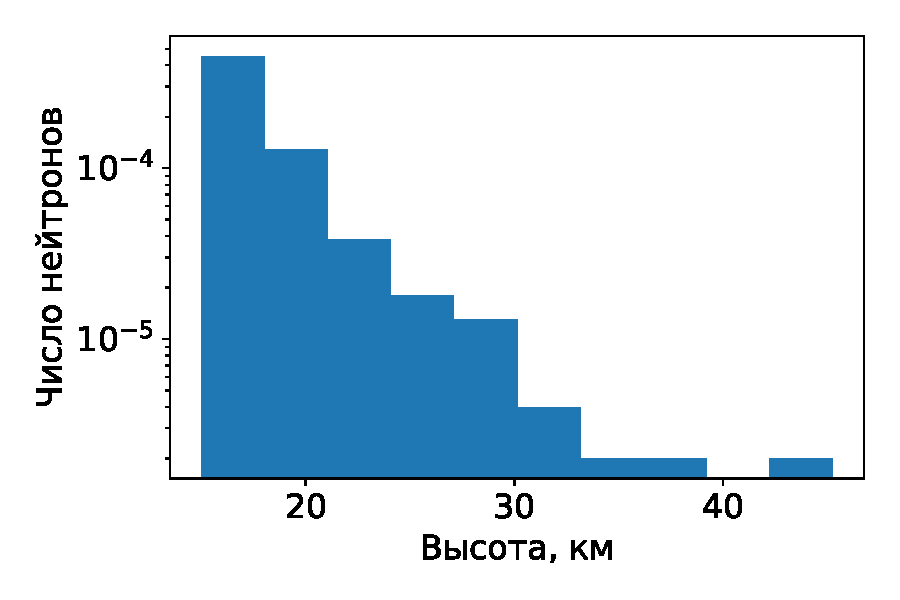
\includegraphics[width=\linewidth]{thunderstorm/neutron/air_z_15MeV.pdf} \\ а)}
        \end{minipage}
        \hfill
        \begin{minipage}[h]{0.49\linewidth}
            \center{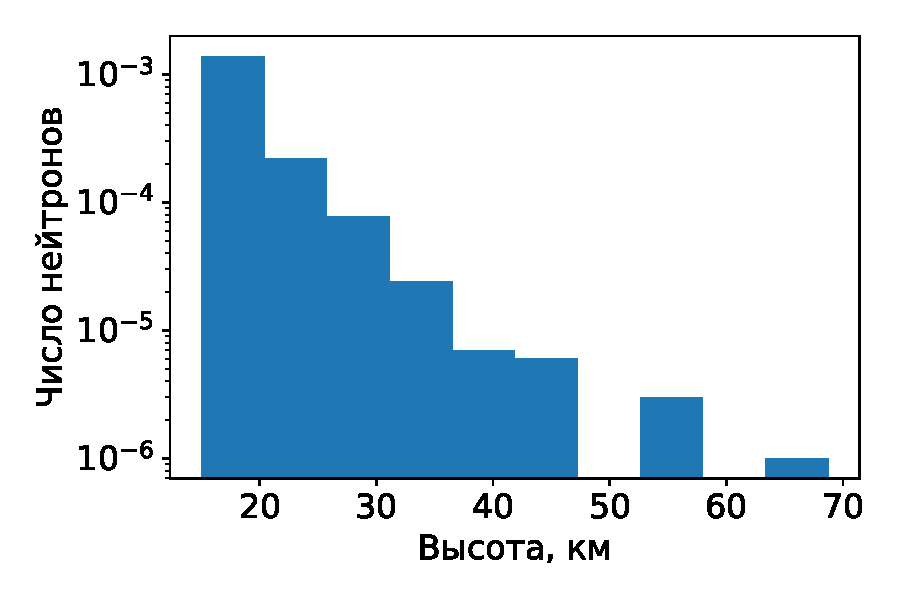
\includegraphics[width=\linewidth]{thunderstorm/neutron/air_z_100MeV.pdf}   \\ б)}
        \end{minipage}
        \caption{Распределение рождения нейтронов по высоте для фотонов с начальной энергией а) 15 МэВ б) 100 МэВ. Нормировано на одну первичную частицу.}
    \end{center}
    \label{fig:storm:neutron_z}
\end{figure}

По результатам моделирования для гамма-квантов с начальной энергией 100 МэВ получено что рождается примерно 1,7 на тысячу гамма-квантов с энергией 100 МэВ. Примерно половина нейтронов имеет энергию до 10 МэВ, вторая часть имеет медленно спадающий спектр в диапазоне от 10 до 70 МэВ. Разброс при рождении в атмосфере достаточно мал, порядка 85 \% нейтронов рождаются в стволе пучка гамма-квантов. Направление импульса рожденных нейтронов имеет достаточно широкий разброс, не позволяющий говорить о наличии выделенного направления движения. График~\ref{fig:storm:neutron_z}а показывает распределение точек рождение нейтронов по высоте. Как мы видим нейтроны рождаются на высотах до 70 километров, далее атмосфера становится сильно разреженной для того что бы шанс с рождения нейтрона был достаточно значительный. Можно отметить что в атмосфере взаимодействует только порядка 0.4 \% гамма-квантов, остальные 99.6\% улетают в космос. Также следует учесть то что гамма-кванты могут рождать нейтроны столкнувшись с корпусом космического аппарата (КА) и телом детектора, однако как показало моделирование, даже если считать что все долетевшие до КА частицы взаимодействуют в нем (что вообще говоря невозможно так как требует КА с массо-габаритным характеристикам значительно превосходящими реальные аппараты), то число таких нейтронов будет составлять только 8\% от числа рожденных в атмосфере.

Результаты моделирования для гамма-квантов с начальной энергией 15 МэВ в целом аналогичны, число рожденных нейтронов примерно в три раза меньше чем для 100 МэВ гаммы, они рождаются на высотах до 40 км (график распределения по высоте приведена на рис.~\ref{fig:storm:neutron_z}б). Только 5\% таких гамма-квантов долетает до космоса, и они не выбывают нейтроны с детектора в КА. Вопрос о достижимости детектора на КА рожденными в атмосфере нейтронов  является дискуссионным, простое GEANT4 моделирование показывает достаточно быструю потерю энергии быстрыми нейтронами, однако есть сомнения в точности выбранной модели, также есть работы показывающий что при больших потоков гамма-квантов возможно достижение нейтронами высот больших 400 км (ссылка а чувака). Однако те не менее моделирование показывает что число нейтронов будет не значительным и размещение детектора нейтронов на КА является не целесообразным и гораздо более эффективным является работа по  регистрации непосредственно гамма-квантов которые долетают до КА в больших количествах.


\section{Reactor like TGE-model}\label{sec:thunderstorm/reactor}

Общим недостатком рассмотренных выше моделей является упрощенная модель электрического поля: оно считается однородным по величине и направлению, что очевидно не так и в полу должны присутствовать разного рода неоднородности, вызванные как краевыми эффектами, так и возникновением сложных конфигураций зарядов. Точное моделирование и анализ динамики лавин убегающих электронов представляет собой сложную задачу, поэтому рассмотрим упрощенную модель что бы оценить потенциальные результаты, которые могут принести исследования в данном направлении. 

Чем ситуация в неоднородном по направлению поле отличается от развития лавин в однородном поле? Когда поле однородно то если гамма-кванты рождают новые затравочные электроны, то лавины от этих электронов будут направлены в том же направлении что и  первая лавина, но при этом их вершина будет смещена к  краю облака, что будет постепенно приводить к затуханию (как показано в предыдущих главах). Если же поле неоднородно по направлению, то направление новых лавин зависит от локальной конфигурации поля и таким образом может возникнуть ситуация изображенная на рисунке --- гамма-кванты от первичной лавины "зажигают" новые локальные ускоряющие ячейки, которые генерирует гамма кванты с угловым распределение значительно развернутым относительно углового распределения исходной лавины, что способствует более равномерному распределению новых затравочных электронов по облаку и как следствие  самоподдерживающей генерации лавин убегающих электронов.
Что бы смоделировать этот процесс, мы рассмотрим такую модель:
\begin{itemize}
    \item  Электронная лавина не рассматривается детально, работает только как ускоряющая ячейка которая 
\end{itemize}
\begin{figure}
    \centering
    \begin{overpic}[scale=.5]{thunderstorm/rltge/electric_streams.pdf}
        \put(15,53){\includegraphics[scale=.015]{thunderstorm/rltge/cell.pdf}}
        \put(20,69){\text{Ускоряющая ячейка}}
        \put(10,10){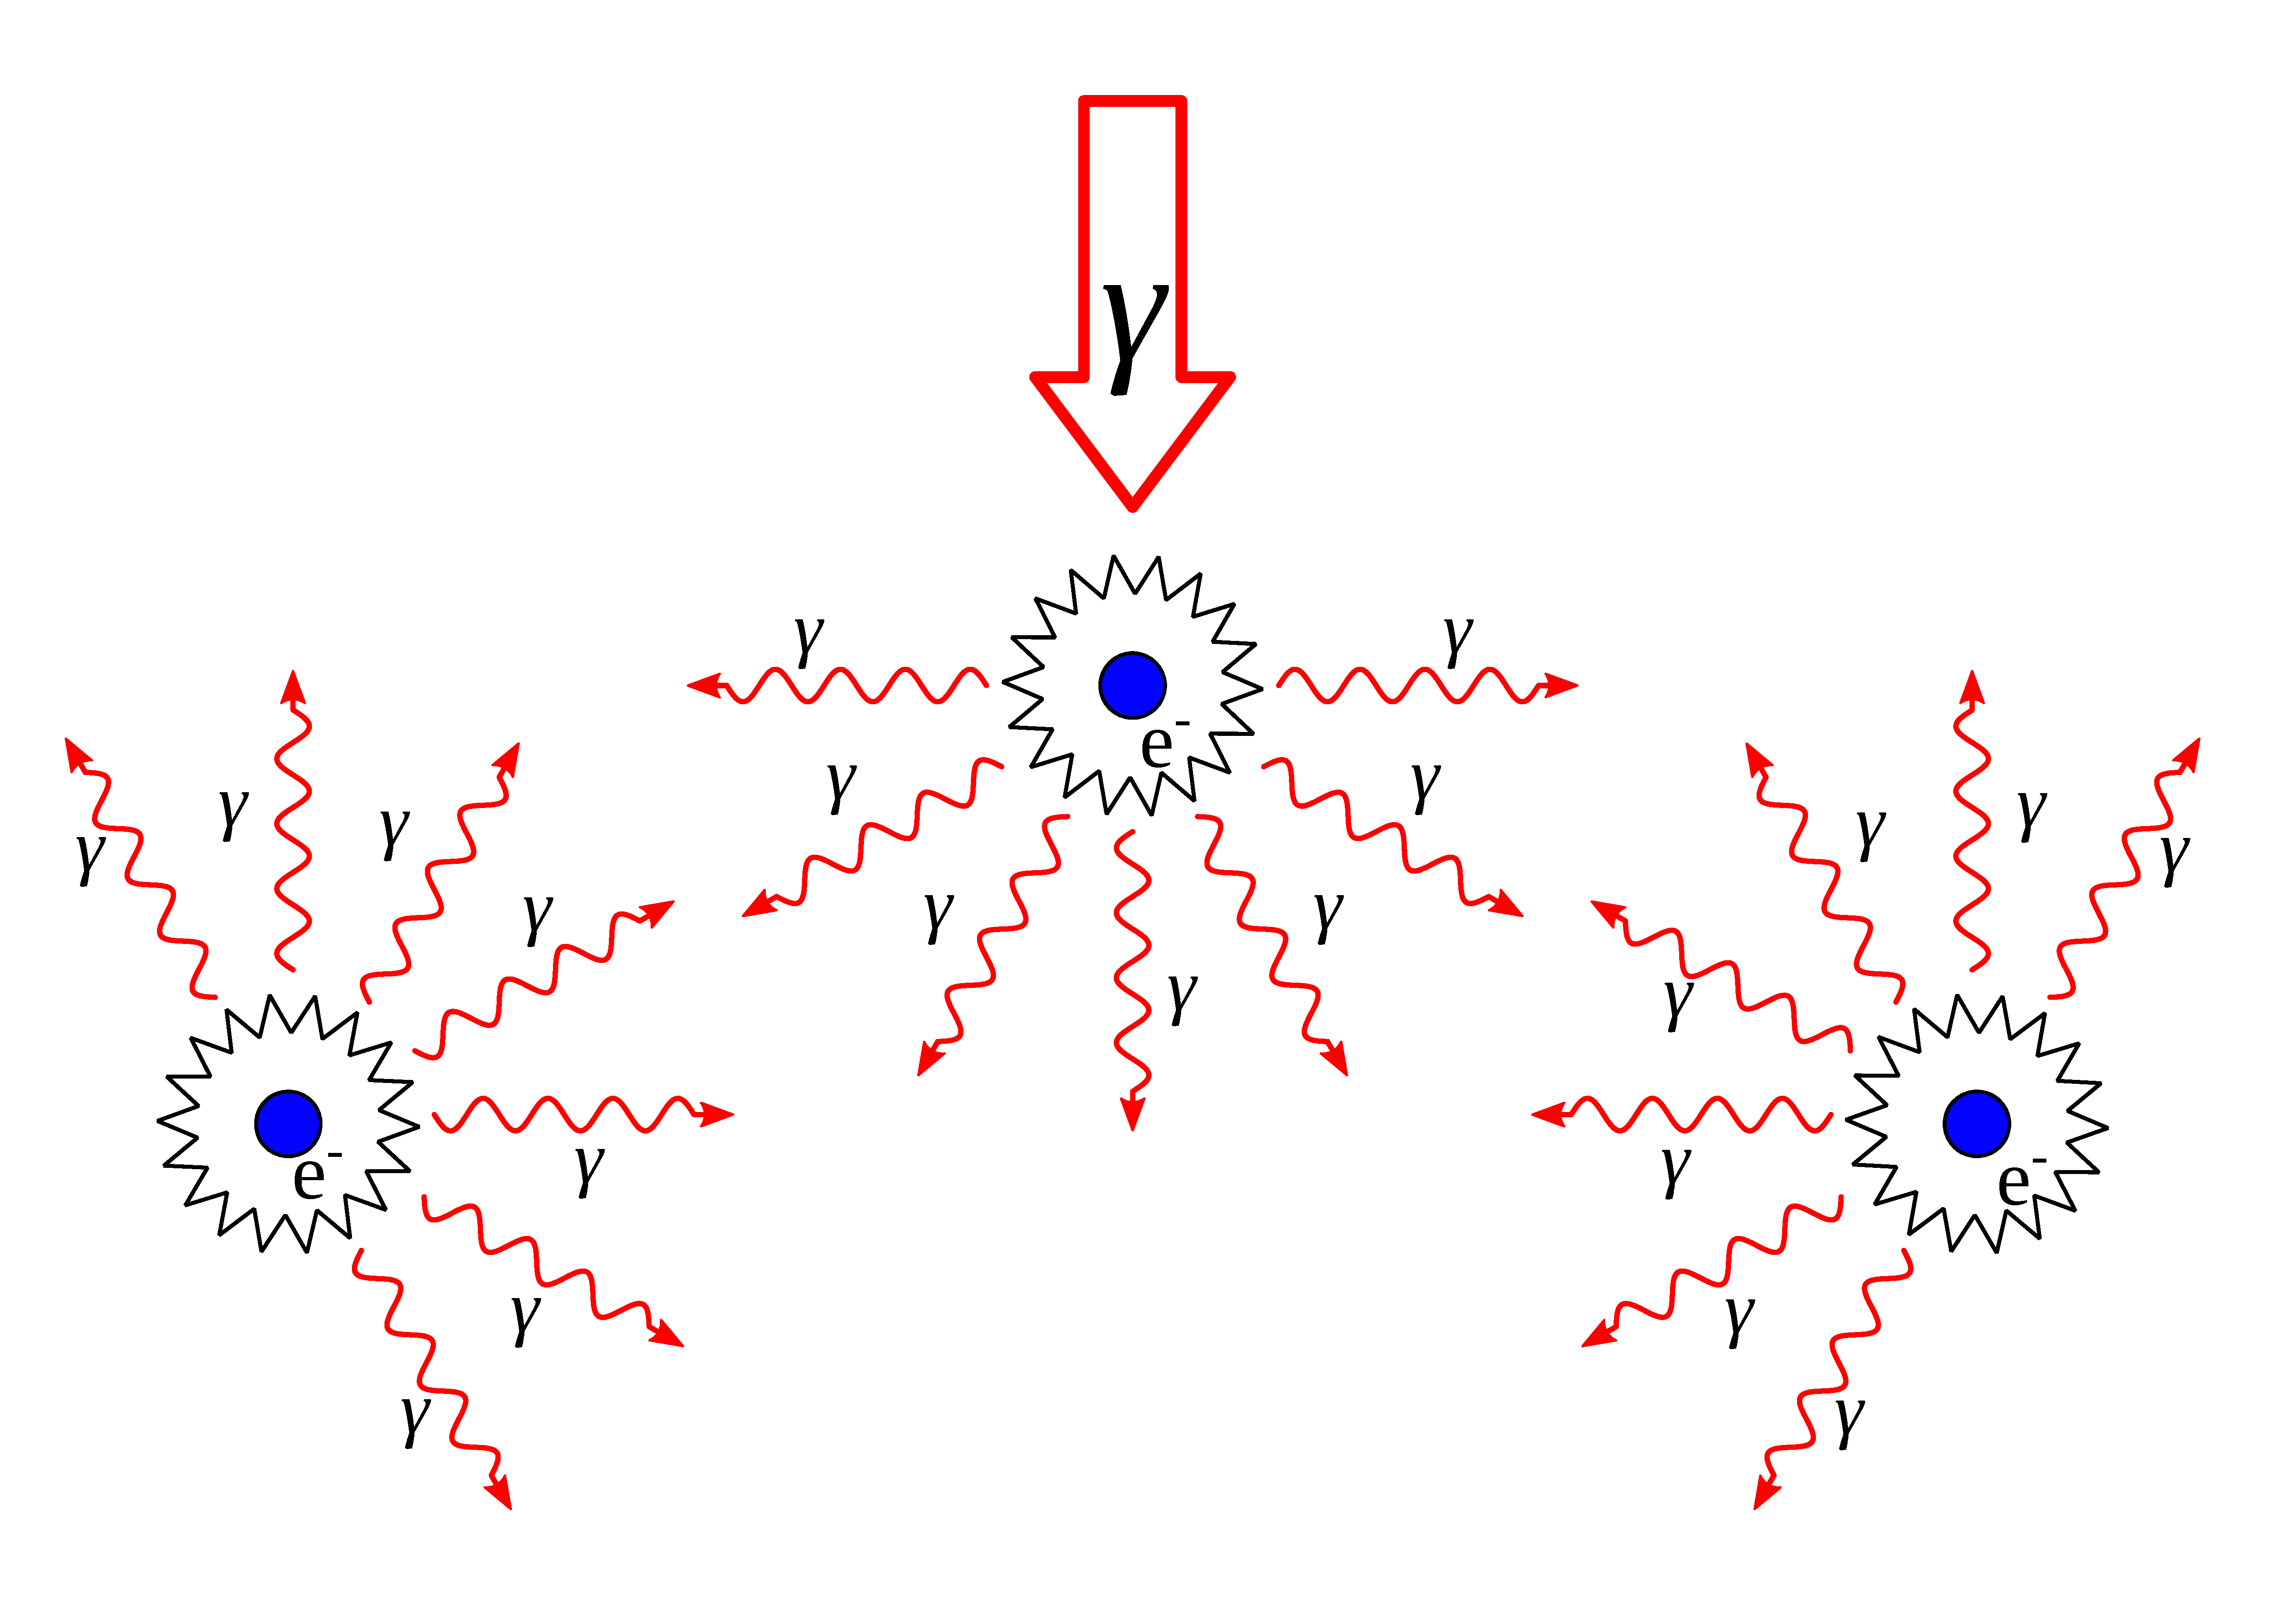
\includegraphics[scale=.15]{thunderstorm/rltge/draw.pdf}}
    \end{overpic}
    \caption{
        Processes occurring in the RL-TGE model: gamma quanta run local acceleration processes in different parts of the cloud with a multidirectional electric field.
    }
    \label{fig:rl}
\end{figure}


\begin{figure}[t]
    \begin{center}
        \begin{minipage}[h]{0.49\linewidth}
            \center{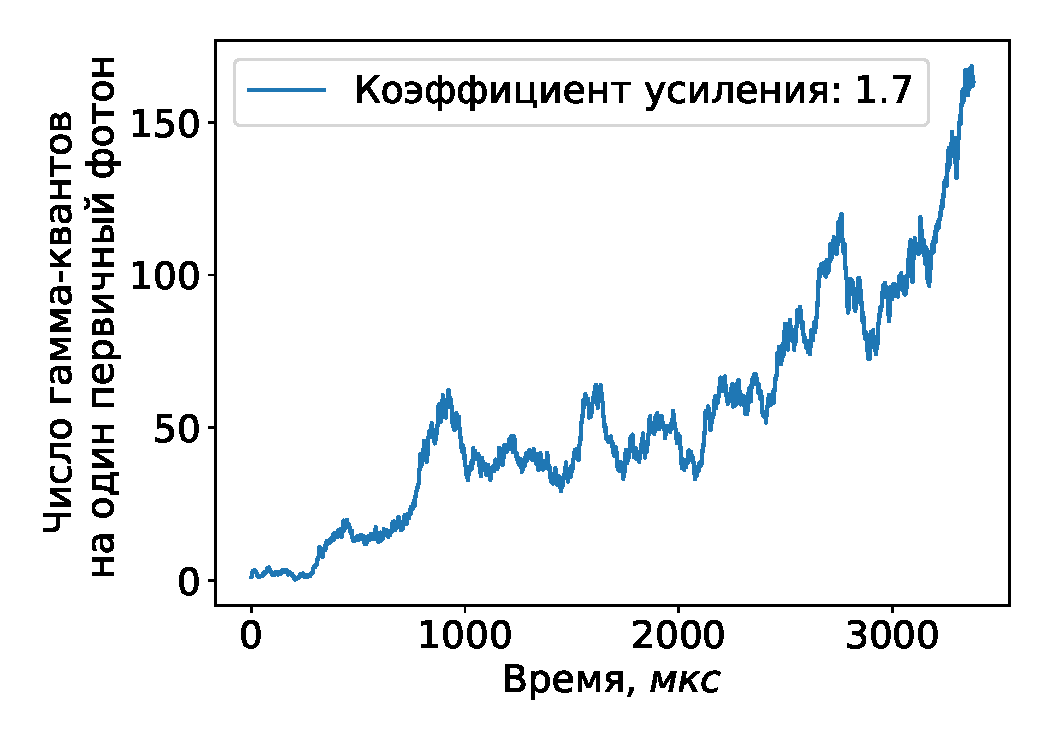
\includegraphics[width=\linewidth]{thunderstorm/RL_proofTGE.pdf} \\ а)}
        \end{minipage}
        \hfill
        \begin{minipage}[h]{0.49\linewidth}
            \center{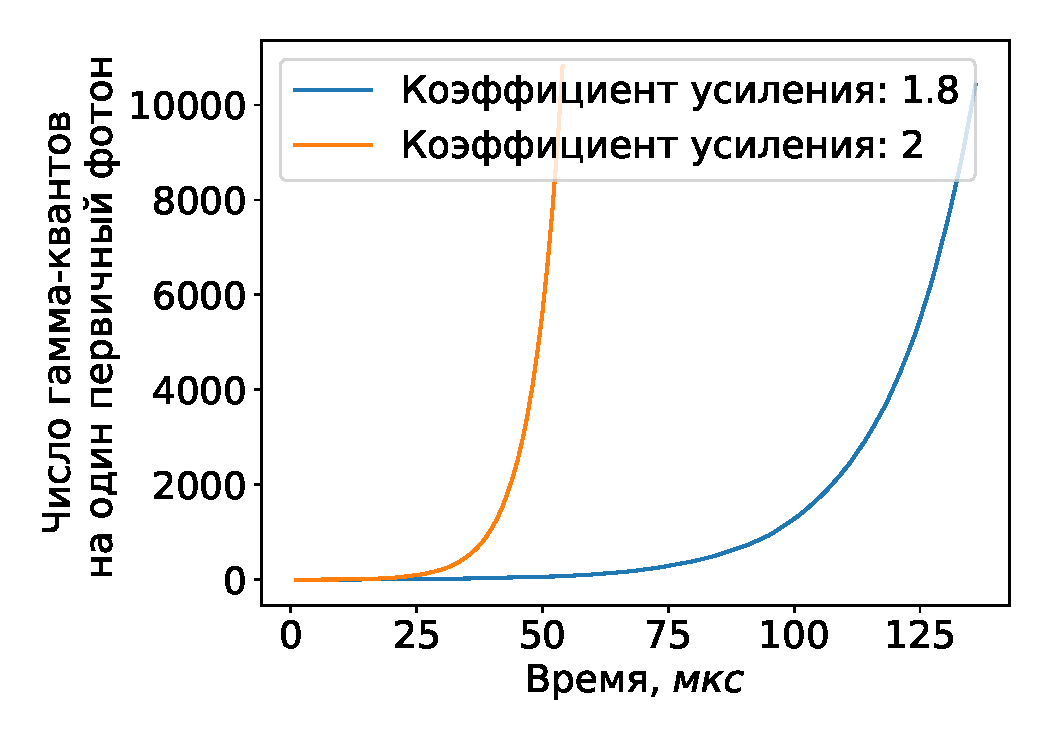
\includegraphics[width=\linewidth]{thunderstorm/RL_proofTGF.pdf}   \\ б)}
        \end{minipage}
        \caption{а) TGE-подобное нарастание. б) TGF-подобное нарастание.}
    \end{center}
    \label{thunder:rl_1}
\end{figure}


\begin{figure}[t]
    \begin{center}
        \begin{minipage}[h]{0.49\linewidth}
            \center{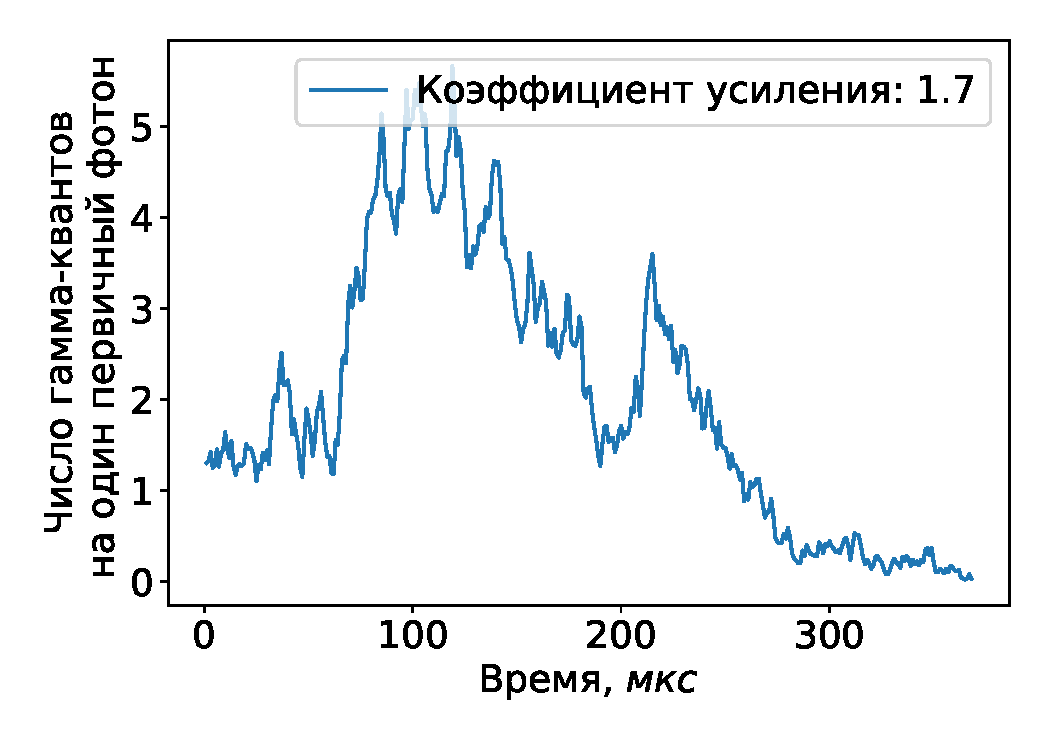
\includegraphics[width=\linewidth]{thunderstorm/RL_Extinction.pdf} \\ а)}
        \end{minipage}
        \hfill
        \begin{minipage}[h]{0.49\linewidth}
            \center{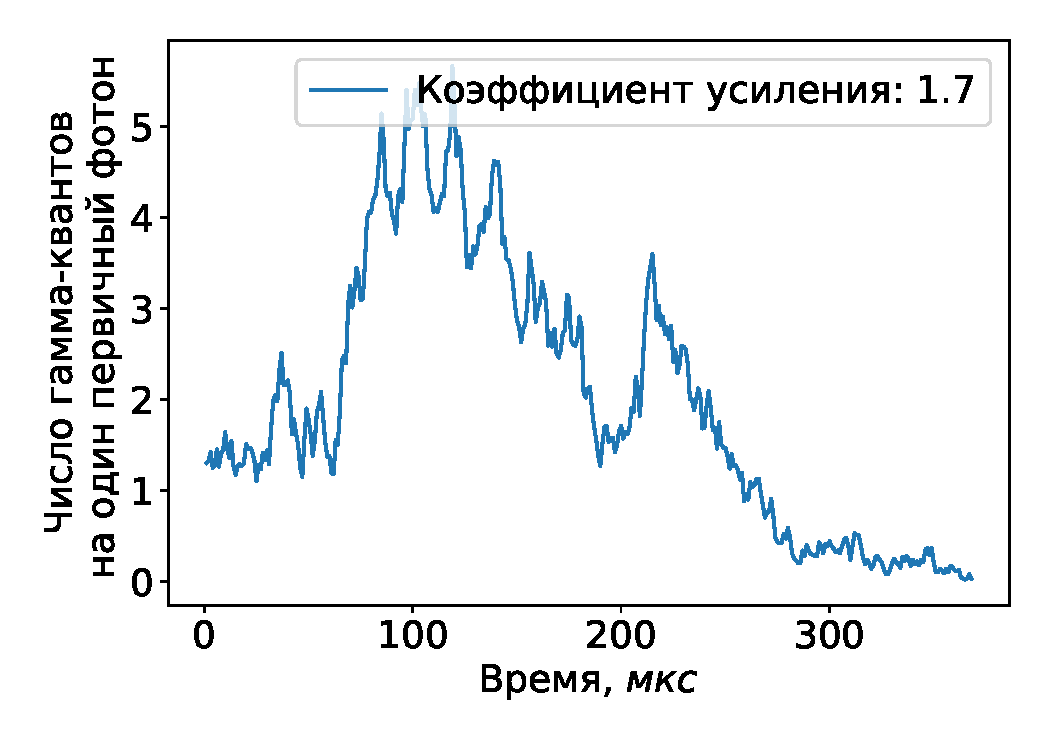
\includegraphics[width=\linewidth]{thunderstorm/RL_Extinction.pdf}   \\ б)}
        \end{minipage}
        \caption{а) Затухание лавины. б) placeholder.}
    \end{center}
    \label{thunder:rl_2}
\end{figure}

\clearpage